% Отчёт по лабораторной работе №3
% «Матрицы в 3D-графике»

\chapter{Ход выполнения работы}

\section{Построение куба в пространстве}

<<<<<<< HEAD
Для начала реализуем построение куба в трёхмерном пространстве с помощью MATLAB. 
=======
Используем код python для выполнения заданий.
>>>>>>> 153dd74 (manual report task 1)

\textbf{Краткое описание алгоритма:}
\begin{enumerate}
<<<<<<< HEAD
    \item \texttt{verticesCube} --- содержит координаты восьми вершин куба: строки соответствуют координатам $x$, $y$, $z$ и однородной координате $w=1$.
    \item \texttt{facesCube} --- определяет, какие вершины соединяются для формирования граней (по четыре индекса на каждую грань).
    \item \texttt{DrawShape} --- функция для визуализации фигуры, использующая команду \texttt{patch} для построения граней. Для перехода к обычным координатам используется деление первых трёх строк на $w$.
\end{enumerate}

\textbf{Зачем нужны однородные координаты?}

Введение четвёртой компоненты ($w$) позволяет удобно описывать аффинные преобразования (масштаб, сдвиг, поворот) в виде матричного умножения. Если $w=1$, то точка находится в обычном 3D-пространстве, а для получения координат достаточно разделить $x$, $y$, $z$ на $w$.
=======
    \item Функция \texttt{create\_cube()} возвращает массив координат 8 вершин куба с центром в начале координат и длиной ребра 2.
    \item Функция \texttt{get\_faces()} задаёт список граней куба через индексы вершин.
    \item Для визуализации используется функция \texttt{plot\_cube}, которая строит грани куба с помощью \texttt{Poly3DCollection} из библиотеки matplotlib.
    \item Для корректного отображения куба в 3D устанавливается одинаковый масштаб по всем осям с помощью функции \texttt{set\_axes\_equal}.
    \item Вся визуализация и сохранение графика выполняется в основной части программы через matplotlib.
\end{enumerate}


\textbf{Зачем использовать четырехкомпонентный вектор?}

Четырехкомпонентный вектор (где последняя координата $w$) позволяет удобно записывать любые аффинные преобразования — такие как перенос, масштабирование и поворот — в виде одного матричного умножения. Благодаря этому все преобразования можно объединять и применять последовательно, не переходя к разным формулам для разных типов операций. После применения преобразования для получения обычных координат достаточно разделить $x$, $y$, $z$ на $w$ (если $w \neq 1$).
>>>>>>> 153dd74 (manual report task 1)

\textbf{Как задать другие фигуры?}

Для построения других многогранников достаточно изменить содержимое матриц \texttt{vertices} и \texttt{faces}.

\begin{figure}[h!]
    \centering
    %\includegraphics[width=0.5\textwidth]{cube1.png}
    \caption{Пример: куб в трёхмерном пространстве}
\end{figure}

\begin{figure}[h!]
    \centering
    %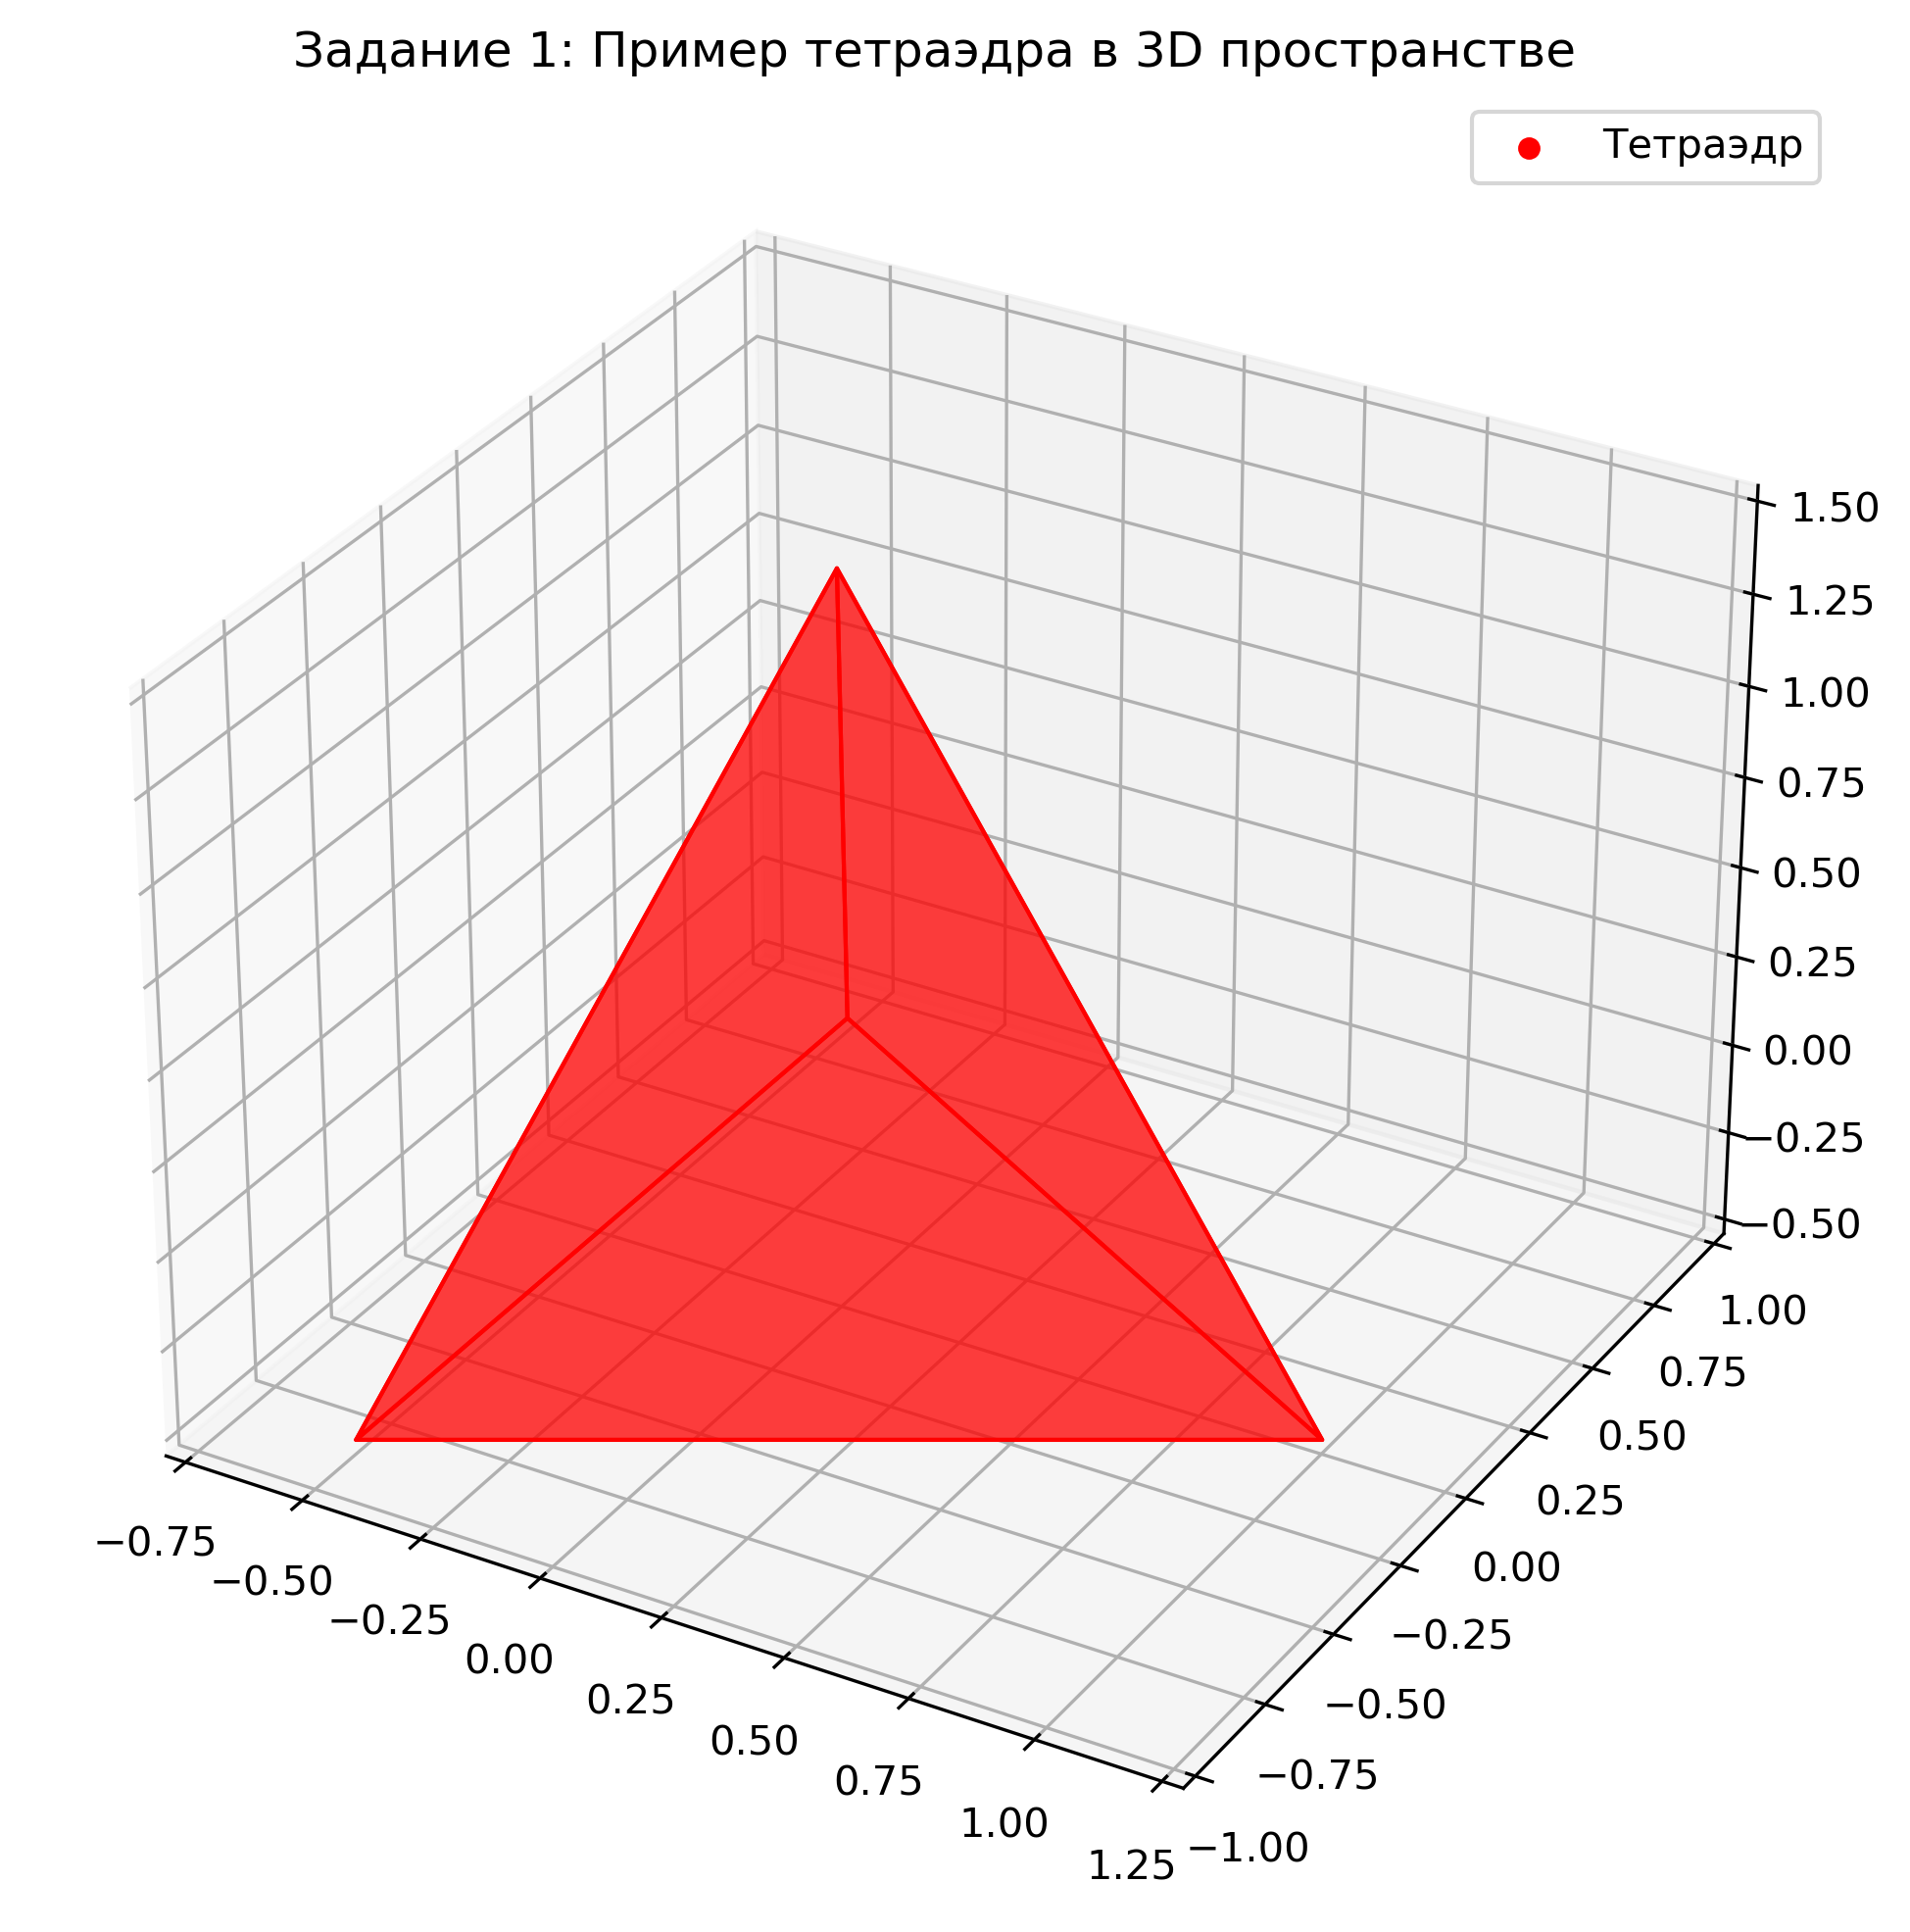
\includegraphics[width=0.5\textwidth]{tetrahedron.png}
    \caption{Пример: тетраэдр в трёхмерном пространстве}
\end{figure}

\section{Масштабирование куба}

Для изменения размеров куба используется матрица масштабирования:
\[
S = \begin{bmatrix}
    s_x & 0 & 0 & 0 \\
    0 & s_y & 0 & 0 \\
    0 & 0 & s_z & 0 \\
    0 & 0 & 0 & 1
\end{bmatrix}
\]
Здесь $s_x$, $s_y$, $s_z$ --- коэффициенты масштабирования по осям $X$, $Y$, $Z$ соответственно. Применяя $S$ к координатам вершин, получаем увеличенный или уменьшенный куб.

\begin{figure}[h!]
    \centering
    %\includegraphics[width=0.5\textwidth]{cube_scale1.png}
    \caption{Исходный куб}
\end{figure}

\begin{figure}[h!]
    \centering
    %\includegraphics[width=0.5\textwidth]{cube_scale2.png}
    \caption{Масштабированный куб}
\end{figure}

\begin{figure}[h!]
    \centering
    %\includegraphics[width=0.5\textwidth]{cube_scale3.png}
    \caption{Куб после уменьшения}
\end{figure}

\section{Смещение (перенос) куба}

Для перемещения объекта в пространстве используется матрица сдвига:
\[
T = \begin{bmatrix}
    1 & 0 & 0 & t_x \\
    0 & 1 & 0 & t_y \\
    0 & 0 & 1 & t_z \\
    0 & 0 & 0 & 1
\end{bmatrix}
\]
Здесь $t_x$, $t_y$, $t_z$ --- величины смещения по соответствующим осям. Итоговые координаты получаются умножением $T$ на вектор вершин.

\begin{figure}[h!]
    \centering
    %\includegraphics[width=0.5\textwidth]{cube_translate1.png}
    \caption{Кубы с разными размерами и положением}
\end{figure}

\textbf{Пояснения к коду:}
\begin{enumerate}
    \item \texttt{verticesCube}, \texttt{facesCube} --- определяют форму и грани.
    \item \texttt{scaleMatrix} --- масштабирует куб.
    \item \texttt{translationMatrix} --- сдвигает куб.
    \item \texttt{combinedMatrix} --- объединяет оба преобразования.
    \item \texttt{DrawShape} --- визуализирует результат.
\end{enumerate}

\section{Поворот куба}

Для поворота используются стандартные матрицы вращения вокруг осей:
\begin{itemize}
    \item \textbf{Вокруг $X$:}
    \[
    R_x(\theta) = \begin{bmatrix}
        1 & 0 & 0 & 0 \\
        0 & \cos\theta & -\sin\theta & 0 \\
        0 & \sin\theta & \cos\theta & 0 \\
        0 & 0 & 0 & 1
    \end{bmatrix}
    \]
    \item \textbf{Вокруг $Y$:}
    \[
    R_y(\theta) = \begin{bmatrix}
        \cos\theta & 0 & \sin\theta & 0 \\
        0 & 1 & 0 & 0 \\
        -\sin\theta & 0 & \cos\theta & 0 \\
        0 & 0 & 0 & 1
    \end{bmatrix}
    \]
    \item \textbf{Вокруг $Z$:}
    \[
    R_z(\theta) = \begin{bmatrix}
        \cos\theta & -\sin\theta & 0 & 0 \\
        \sin\theta & \cos\theta & 0 & 0 \\
        0 & 0 & 1 & 0 \\
        0 & 0 & 0 & 1
    \end{bmatrix}
    \]
\end{itemize}

\begin{figure}[h!]
    \centering
    %\includegraphics[width=0.5\textwidth]{cube_rotate1.png}
    \caption{Куб после поворота}
\end{figure}

\begin{figure}[h!]
    \centering
    %\includegraphics[width=0.5\textwidth]{cube_rotate2.png}
    \caption{Поворот куба вокруг другой оси}
\end{figure}

\begin{figure}[h!]
    \centering
    %\includegraphics[width=0.5\textwidth]{cube_rotate3.png}
    \caption{Комбинированный поворот}
\end{figure}

В отличие от двумерного случая, в 3D-поворотах важен порядок применения матриц: результат зависит от последовательности вращений.

\section{Поворот куба вокруг вершины}

Чтобы повернуть куб относительно одной из его вершин, нужно:
\begin{enumerate}
    \item Сначала сдвинуть куб так, чтобы выбранная вершина совпала с началом координат.
    \item Применить матрицу вращения.
    \item Вернуть куб обратно обратным сдвигом.
\end{enumerate}

\begin{figure}[h!]
    \centering
    %\includegraphics[width=0.5\textwidth]{vertex_rotate.png}
    \caption{Поворот куба вокруг вершины}
\end{figure}

\section{Виртуальная камера}

Для имитации движения камеры сцены используются матрицы вращения (как выше) и матрица переноса камеры:
\[
T_{camera} = \begin{bmatrix}
1 & 0 & 0 & -t_x \\
0 & 1 & 0 & -t_y \\
0 & 0 & 1 & -t_z \\
0 & 0 & 0 & 1
\end{bmatrix}
\]
Здесь $t_x$, $t_y$, $t_z$ --- положение камеры. Отрицательный знак означает, что движение камеры в одну сторону эквивалентно движению сцены в противоположную.

\begin{figure}[h!]
    \centering
    %\includegraphics[width=0.5\textwidth]{camera1.png}
    \caption{Сцена с несколькими кубами и виртуальной камерой}
\end{figure}

\begin{figure}[h!]
    \centering
    %\includegraphics[width=0.5\textwidth]{camera2.png}
    \caption{Вид сцены под другим углом}
\end{figure}

Обратная матрица позволяет вернуть камеру в исходное положение.

\section{Перспективное отображение}

Для создания эффекта перспективы используется специальная матрица проекции:
\[
M_{proj} = \begin{bmatrix}
s & 0 & 0 & 0 \\
0 & s & 0 & 0 \\
0 & 0 & \frac{f+ n}{f-n} & -1 \\
0 & 0 & \frac{2fn}{f-n} & 0
\end{bmatrix}
\]
Параметры:
\begin{itemize}
    \item $s = \frac{1}{\tan(\frac{\text{fov}}{2})}$ --- масштаб по $X$ и $Y$ (fov --- угол обзора).
    \item $f$, $n$ --- дальняя и ближняя плоскости отсечения.
    \item Остальные элементы отвечают за нормализацию глубины и перспективу.
\end{itemize}

\begin{figure}[h!]
    \centering
    %\includegraphics[width=0.5\textwidth]{perspective1.png}
    \caption{Перспективное отображение сцены}
\end{figure}

\textbf{Пояснения:}

Такая матрица позволяет корректно отображать удалённые объекты меньшими, чем ближние, и задаёт параметры видимости сцены (угол обзора, глубина, соотношение сторон).

\section{Выводы}

В ходе работы были реализованы и исследованы основные преобразования в 3D: масштабирование, перенос, поворот, а также перспективная проекция и виртуальная камера. Показано, как с помощью матриц можно гибко управлять положением и видом объектов в пространстве, а также формировать реалистичное изображение сцены.
